
%% bare_jrnl.tex
%% V1.3
%% 2007/01/11
%% by Michael Shell
%% see http://www.michaelshell.org/
%% for current contact information.
%%
%% This is a skeleton file demonstrating the use of IEEEtran.cls
%% (requires IEEEtran.cls version 1.7 or later) with an IEEE journal paper.
%%
%% Support sites:
%% http://www.michaelshell.org/tex/ieeetran/
%% http://www.ctan.org/tex-archive/macros/latex/contrib/IEEEtran/
%% and
%% http://www.ieee.org/



% *** Authors should verify (and, if needed, correct) their LaTeX system  ***
% *** with the testflow diagnostic prior to trusting their LaTeX platform ***
% *** with production work. IEEE's font choices can trigger bugs that do  ***
% *** not appear when using other class files.                            ***
% The testflow support page is at:
% http://www.michaelshell.org/tex/testflow/


%%*************************************************************************
%% Legal Notice:
%% This code is offered as-is without any warranty either expressed or
%% implied; without even the implied warranty of MERCHANTABILITY or
%% FITNESS FOR A PARTICULAR PURPOSE! 
%% User assumes all risk.
%% In no event shall IEEE or any contributor to this code be liable for
%% any damages or losses, including, but not limited to, incidental,
%% consequential, or any other damages, resulting from the use or misuse
%% of any information contained here.
%%
%% All comments are the opinions of their respective authors and are not
%% necessarily endorsed by the IEEE.
%%
%% This work is distributed under the LaTeX Project Public License (LPPL)
%% ( http://www.latex-project.org/ ) version 1.3, and may be freely used,
%% distributed and modified. A copy of the LPPL, version 1.3, is included
%% in the base LaTeX documentation of all distributions of LaTeX released
%% 2003/12/01 or later.
%% Retain all contribution notices and credits.
%% ** Modified files should be clearly indicated as such, including  **
%% ** renaming them and changing author support contact information. **
%%
%% File list of work: IEEEtran.cls, IEEEtran_HOWTO.pdf, bare_adv.tex,
%%                    bare_conf.tex, bare_jrnl.tex, bare_jrnl_compsoc.tex
%%*************************************************************************

% Note that the a4paper option is mainly intended so that authors in
% countries using A4 can easily print to A4 and see how their papers will
% look in print - the typesetting of the document will not typically be
% affected with changes in paper size (but the bottom and side margins will).
% Use the testflow package mentioned above to verify correct handling of
% both paper sizes by the user's LaTeX system.
%
% Also note that the "draftcls" or "draftclsnofoot", not "draft", option
% should be used if it is desired that the figures are to be displayed in
% draft mode.
%
\documentclass[journal]{IEEEtran}
\usepackage{blindtext}
\usepackage{graphicx}
\usepackage{amsthm}
\usepackage{amsfonts}
\usepackage{amsmath}
\newtheorem{mydef}{Definition}

% Some very useful LaTeX packages include:
% (uncomment the ones you want to load)


% *** MISC UTILITY PACKAGES ***
%
%\usepackage{ifpdf}
% Heiko Oberdiek's ifpdf.sty is very useful if you need conditional
% compilation based on whether the output is pdf or dvi.
% usage:
% \ifpdf
%   % pdf code
% \else
%   % dvi code
% \fi
% The latest version of ifpdf.sty can be obtained from:
% http://www.ctan.org/tex-archive/macros/latex/contrib/oberdiek/
% Also, note that IEEEtran.cls V1.7 and later provides a builtin
% \ifCLASSINFOpdf conditional that works the same way.
% When switching from latex to pdflatex and vice-versa, the compiler may
% have to be run twice to clear warning/error messages.






% *** CITATION PACKAGES ***
%
%\usepackage{cite}
% cite.sty was written by Donald Arseneau
% V1.6 and later of IEEEtran pre-defines the format of the cite.sty package
% \cite{} output to follow that of IEEE. Loading the cite package will
% result in citation numbers being automatically sorted and properly
% "compressed/ranged". e.g., [1], [9], [2], [7], [5], [6] without using
% cite.sty will become [1], [2], [5]--[7], [9] using cite.sty. cite.sty's
% \cite will automatically add leading space, if needed. Use cite.sty's
% noadjust option (cite.sty V3.8 and later) if you want to turn this off.
% cite.sty is already installed on most LaTeX systems. Be sure and use
% version 4.0 (2003-05-27) and later if using hyperref.sty. cite.sty does
% not currently provide for hyperlinked citations.
% The latest version can be obtained at:
% http://www.ctan.org/tex-archive/macros/latex/contrib/cite/
% The documentation is contained in the cite.sty file itself.






% *** GRAPHICS RELATED PACKAGES ***
%
\ifCLASSINFOpdf
  % \usepackage[pdftex]{graphicx}
  % declare the path(s) where your graphic files are
  % \graphicspath{{../pdf/}{../jpeg/}}
  % and their extensions so you won't have to specify these with
  % every instance of \includegraphics
  % \DeclareGraphicsExtensions{.pdf,.jpeg,.png}
\else
  % or other class option (dvipsone, dvipdf, if not using dvips). graphicx
  % will default to the driver specified in the system graphics.cfg if no
  % driver is specified.
  % \usepackage[dvips]{graphicx}
  % declare the path(s) where your graphic files are
  % \graphicspath{{../eps/}}
  % and their extensions so you won't have to specify these with
  % every instance of \includegraphics
  % \DeclareGraphicsExtensions{.eps}
\fi
% graphicx was written by David Carlisle and Sebastian Rahtz. It is
% required if you want graphics, photos, etc. graphicx.sty is already
% installed on most LaTeX systems. The latest version and documentation can
% be obtained at: 
% http://www.ctan.org/tex-archive/macros/latex/required/graphics/
% Another good source of documentation is "Using Imported Graphics in
% LaTeX2e" by Keith Reckdahl which can be found as epslatex.ps or
% epslatex.pdf at: http://www.ctan.org/tex-archive/info/
%
% latex, and pdflatex in dvi mode, support graphics in encapsulated
% postscript (.eps) format. pdflatex in pdf mode supports graphics
% in .pdf, .jpeg, .png and .mps (metapost) formats. Users should ensure
% that all non-photo figures use a vector format (.eps, .pdf, .mps) and
% not a bitmapped formats (.jpeg, .png). IEEE frowns on bitmapped formats
% which can result in "jaggedy"/blurry rendering of lines and letters as
% well as large increases in file sizes.
%
% You can find documentation about the pdfTeX application at:
% http://www.tug.org/applications/pdftex





% *** MATH PACKAGES ***
%
%\usepackage[cmex10]{amsmath}
% A popular package from the American Mathematical Society that provides
% many useful and powerful commands for dealing with mathematics. If using
% it, be sure to load this package with the cmex10 option to ensure that
% only type 1 fonts will utilized at all point sizes. Without this option,
% it is possible that some math symbols, particularly those within
% footnotes, will be rendered in bitmap form which will result in a
% document that can not be IEEE Xplore compliant!
%
% Also, note that the amsmath package sets \interdisplaylinepenalty to 10000
% thus preventing page breaks from occurring within multiline equations. Use:
%\interdisplaylinepenalty=2500
% after loading amsmath to restore such page breaks as IEEEtran.cls normally
% does. amsmath.sty is already installed on most LaTeX systems. The latest
% version and documentation can be obtained at:
% http://www.ctan.org/tex-archive/macros/latex/required/amslatex/math/





% *** SPECIALIZED LIST PACKAGES ***
%
%\usepackage{algorithmic}
% algorithmic.sty was written by Peter Williams and Rogerio Brito.
% This package provides an algorithmic environment fo describing algorithms.
% You can use the algorithmic environment in-text or within a figure
% environment to provide for a floating algorithm. Do NOT use the algorithm
% floating environment provided by algorithm.sty (by the same authors) or
% algorithm2e.sty (by Christophe Fiorio) as IEEE does not use dedicated
% algorithm float types and packages that provide these will not provide
% correct IEEE style captions. The latest version and documentation of
% algorithmic.sty can be obtained at:
% http://www.ctan.org/tex-archive/macros/latex/contrib/algorithms/
% There is also a support site at:
% http://algorithms.berlios.de/index.html
% Also of interest may be the (relatively newer and more customizable)
% algorithmicx.sty package by Szasz Janos:
% http://www.ctan.org/tex-archive/macros/latex/contrib/algorithmicx/




% *** ALIGNMENT PACKAGES ***
%
%\usepackage{array}
% Frank Mittelbach's and David Carlisle's array.sty patches and improves
% the standard LaTeX2e array and tabular environments to provide better
% appearance and additional user controls. As the default LaTeX2e table
% generation code is lacking to the point of almost being broken with
% respect to the quality of the end results, all users are strongly
% advised to use an enhanced (at the very least that provided by array.sty)
% set of table tools. array.sty is already installed on most systems. The
% latest version and documentation can be obtained at:
% http://www.ctan.org/tex-archive/macros/latex/required/tools/


%\usepackage{mdwmath}
%\usepackage{mdwtab}
% Also highly recommended is Mark Wooding's extremely powerful MDW tools,
% especially mdwmath.sty and mdwtab.sty which are used to format equations
% and tables, respectively. The MDWtools set is already installed on most
% LaTeX systems. The lastest version and documentation is available at:
% http://www.ctan.org/tex-archive/macros/latex/contrib/mdwtools/


% IEEEtran contains the IEEEeqnarray family of commands that can be used to
% generate multiline equations as well as matrices, tables, etc., of high
% quality.


%\usepackage{eqparbox}
% Also of notable interest is Scott Pakin's eqparbox package for creating
% (automatically sized) equal width boxes - aka "natural width parboxes".
% Available at:
% http://www.ctan.org/tex-archive/macros/latex/contrib/eqparbox/





% *** SUBFIGURE PACKAGES ***
%\usepackage[tight,footnotesize]{subfigure}
% subfigure.sty was written by Steven Douglas Cochran. This package makes it
% easy to put subfigures in your figures. e.g., "Figure 1a and 1b". For IEEE
% work, it is a good idea to load it with the tight package option to reduce
% the amount of white space around the subfigures. subfigure.sty is already
% installed on most LaTeX systems. The latest version and documentation can
% be obtained at:
% http://www.ctan.org/tex-archive/obsolete/macros/latex/contrib/subfigure/
% subfigure.sty has been superceeded by subfig.sty.



%\usepackage[caption=false]{caption}
%\usepackage[font=footnotesize]{subfig}
% subfig.sty, also written by Steven Douglas Cochran, is the modern
% replacement for subfigure.sty. However, subfig.sty requires and
% automatically loads Axel Sommerfeldt's caption.sty which will override
% IEEEtran.cls handling of captions and this will result in nonIEEE style
% figure/table captions. To prevent this problem, be sure and preload
% caption.sty with its "caption=false" package option. This is will preserve
% IEEEtran.cls handing of captions. Version 1.3 (2005/06/28) and later 
% (recommended due to many improvements over 1.2) of subfig.sty supports
% the caption=false option directly:
%\usepackage[caption=false,font=footnotesize]{subfig}
%
% The latest version and documentation can be obtained at:
% http://www.ctan.org/tex-archive/macros/latex/contrib/subfig/
% The latest version and documentation of caption.sty can be obtained at:
% http://www.ctan.org/tex-archive/macros/latex/contrib/caption/




% *** FLOAT PACKAGES ***
%
%\usepackage{fixltx2e}
% fixltx2e, the successor to the earlier fix2col.sty, was written by
% Frank Mittelbach and David Carlisle. This package corrects a few problems
% in the LaTeX2e kernel, the most notable of which is that in current
% LaTeX2e releases, the ordering of single and double column floats is not
% guaranteed to be preserved. Thus, an unpatched LaTeX2e can allow a
% single column figure to be placed prior to an earlier double column
% figure. The latest version and documentation can be found at:
% http://www.ctan.org/tex-archive/macros/latex/base/



%\usepackage{stfloats}
% stfloats.sty was written by Sigitas Tolusis. This package gives LaTeX2e
% the ability to do double column floats at the bottom of the page as well
% as the top. (e.g., "\begin{figure*}[!b]" is not normally possible in
% LaTeX2e). It also provides a command:
%\fnbelowfloat
% to enable the placement of footnotes below bottom floats (the standard
% LaTeX2e kernel puts them above bottom floats). This is an invasive package
% which rewrites many portions of the LaTeX2e float routines. It may not work
% with other packages that modify the LaTeX2e float routines. The latest
% version and documentation can be obtained at:
% http://www.ctan.org/tex-archive/macros/latex/contrib/sttools/
% Documentation is contained in the stfloats.sty comments as well as in the
% presfull.pdf file. Do not use the stfloats baselinefloat ability as IEEE
% does not allow \baselineskip to stretch. Authors submitting work to the
% IEEE should note that IEEE rarely uses double column equations and
% that authors should try to avoid such use. Do not be tempted to use the
% cuted.sty or midfloat.sty packages (also by Sigitas Tolusis) as IEEE does
% not format its papers in such ways.


%\ifCLASSOPTIONcaptionsoff
%  \usepackage[nomarkers]{endfloat}
% \let\MYoriglatexcaption\caption
% \renewcommand{\caption}[2][\relax]{\MYoriglatexcaption[#2]{#2}}
%\fi
% endfloat.sty was written by James Darrell McCauley and Jeff Goldberg.
% This package may be useful when used in conjunction with IEEEtran.cls'
% captionsoff option. Some IEEE journals/societies require that submissions
% have lists of figures/tables at the end of the paper and that
% figures/tables without any captions are placed on a page by themselves at
% the end of the document. If needed, the draftcls IEEEtran class option or
% \CLASSINPUTbaselinestretch interface can be used to increase the line
% spacing as well. Be sure and use the nomarkers option of endfloat to
% prevent endfloat from "marking" where the figures would have been placed
% in the text. The two hack lines of code above are a slight modification of
% that suggested by in the endfloat docs (section 8.3.1) to ensure that
% the full captions always appear in the list of figures/tables - even if
% the user used the short optional argument of \caption[]{}.
% IEEE papers do not typically make use of \caption[]'s optional argument,
% so this should not be an issue. A similar trick can be used to disable
% captions of packages such as subfig.sty that lack options to turn off
% the subcaptions:
% For subfig.sty:
% \let\MYorigsubfloat\subfloat
% \renewcommand{\subfloat}[2][\relax]{\MYorigsubfloat[]{#2}}
% For subfigure.sty:
% \let\MYorigsubfigure\subfigure
% \renewcommand{\subfigure}[2][\relax]{\MYorigsubfigure[]{#2}}
% However, the above trick will not work if both optional arguments of
% the \subfloat/subfig command are used. Furthermore, there needs to be a
% description of each subfigure *somewhere* and endfloat does not add
% subfigure captions to its list of figures. Thus, the best approach is to
% avoid the use of subfigure captions (many IEEE journals avoid them anyway)
% and instead reference/explain all the subfigures within the main caption.
% The latest version of endfloat.sty and its documentation can obtained at:
% http://www.ctan.org/tex-archive/macros/latex/contrib/endfloat/
%
% The IEEEtran \ifCLASSOPTIONcaptionsoff conditional can also be used
% later in the document, say, to conditionally put the References on a 
% page by themselves.





% *** PDF, URL AND HYPERLINK PACKAGES ***
%
%\usepackage{url}
% url.sty was written by Donald Arseneau. It provides better support for
% handling and breaking URLs. url.sty is already installed on most LaTeX
% systems. The latest version can be obtained at:
% http://www.ctan.org/tex-archive/macros/latex/contrib/misc/
% Read the url.sty source comments for usage information. Basically,
% \url{my_url_here}.





% *** Do not adjust lengths that control margins, column widths, etc. ***
% *** Do not use packages that alter fonts (such as pslatex).         ***
% There should be no need to do such things with IEEEtran.cls V1.6 and later.
% (Unless specifically asked to do so by the journal or conference you plan
% to submit to, of course. )


% correct bad hyphenation here
\hyphenation{op-tical net-works semi-conduc-tor}


\begin{document}
%
% paper title
% can use linebreaks \\ within to get better formatting as desired
\title{Master thesis Espose: Conception and Development of Semantic Complex Pattern Mining methods on Event Streams}
%
%
% author names and IEEE memberships
% note positions of commas and nonbreaking spaces ( ~ ) LaTeX will not break
% a structure at a ~ so this keeps an author's name from being broken across
% two lines.
% use \thanks{} to gain access to the first footnote area
% a separate \thanks must be used for each paragraph as LaTeX2e's \thanks
% was not built to handle multiple paragraphs
%

\author{Leon Bornemann, Freie Universit\"at Berlin}

% note the % following the last \IEEEmembership and also \thanks - 
% these prevent an unwanted space from occurring between the last author name
% and the end of the author line. i.e., if you had this:
% 
% \author{....lastname \thanks{...} \thanks{...} }
%                     ^------------^------------^----Do not want these spaces!
%
% a space would be appended to the last name and could cause every name on that
% line to be shifted left slightly. This is one of those "LaTeX things". For
% instance, "\textbf{A} \textbf{B}" will typeset as "A B" not "AB". To get
% "AB" then you have to do: "\textbf{A}\textbf{B}"
% \thanks is no different in this regard, so shield the last } of each \thanks
% that ends a line with a % and do not let a space in before the next \thanks.
% Spaces after \IEEEmembership other than the last one are OK (and needed) as
% you are supposed to have spaces between the names. For what it is worth,
% this is a minor point as most people would not even notice if the said evil
% space somehow managed to creep in.



% The paper headers
\markboth{Master thesis expose}%
{Shell \MakeLowercase{\textit{et al.}}: Bare Demo of IEEEtran.cls for Journals}
% The only time the second header will appear is for the odd numbered pages
% after the title page when using the twoside option.
% 
% *** Note that you probably will NOT want to include the author's ***
% *** name in the headers of peer review papers.                   ***
% You can use \ifCLASSOPTIONpeerreview for conditional compilation here if
% you desire.




% If you want to put a publisher's ID mark on the page you can do it like
% this:
%\IEEEpubid{0000--0000/00\$00.00~\copyright~2007 IEEE}
% Remember, if you use this you must call \IEEEpubidadjcol in the second
% column for its text to clear the IEEEpubid mark.



% use for special paper notices
%\IEEEspecialpapernotice{(Invited Paper)}




% make the title area
\maketitle


\begin{abstract}
This is an expose for the proposed topic
\end{abstract}
% IEEEtran.cls defaults to using nonbold math in the Abstract.
% This preserves the distinction between vectors and scalars. However,
% if the journal you are submitting to favors bold math in the abstract,
% then you can use LaTeX's standard command \boldmath at the very start
% of the abstract to achieve this. Many IEEE journals frown on math
% in the abstract anyway.

% Note that keywords are not normally used for peerreview papers.
\begin{IEEEkeywords}
data mining, semantic pattern mining, event, stream, streaming
\end{IEEEkeywords}






% For peer review papers, you can put extra information on the cover
% page as needed:
% \ifCLASSOPTIONpeerreview
% \begin{center} \bfseries EDICS Category: 3-BBND \end{center}
% \fi
%
% For peerreview papers, this IEEEtran command inserts a page break and
% creates the second title. It will be ignored for other modes.
\IEEEpeerreviewmaketitle



\section{Introduction}
Almost any application domain of information systems has some data that is being generated. Data is available in many different forms. One of these forms are data streams. Data streams are not limited to the recent rise in popularity of video and audio streams. On the contrary the application domains that produce data in the form of streams are very diverse. They include for example constantly running business applications that log business activities and events, sensor networks that report usage data or devices that take measurements of physical quantities (such as temperature, pressure, humidity, etc...) at certain points of time. \newline
The fact that streams generate a constant stream of data and thus lead to a constantly growing database is a significant difference to classic applications of data mining in which there is a static (training) database. Despite that significant difference in the data representation, many fields of interest in the context of static databases remain the same for data streams. Common areas of interest are frequent patterns, predictive patterns, association rules, clustering and classification of the data entities. Approaches and algorithms that solve these problems for static databases, while by no means fully researched, are rather well known and evaluated. Applying these methods to data streams can present challenges and may demand many modifications due to the large and possibly infinite amounts of data produced by streams. Naturally data mining methods for stream data must be especially fast, scalable and memory efficient. \newline
This thesis will focus on the subtopic of episode pattern mining from stream data or very large log files or databases. While mining of frequent episodes has already been looked at (TODO: cite PHD thesis), the suggested algorithms use multiple passes over the database to find all frequent episodes. Multiple passes are often not feasible for large data streams, since it is impossible to store the stream in its entire length and thus impossible to look at it more than once. Additionally the state of the art episode definition is rather restrictive in the context of complex events. It is for example impossible to express disjunctions within episodes. Including additional operators like disjunctions would extend the expressive power of episodes, which means that more complex events can be specified and mined as episodes. However, expanding the expressive power also means that episodes will become more difficult to mine, since there are more potential candidates that the algorithm needs to keep track of. This is where semantic knowledge can come into play. In a realistic scenario, users are not interested in all the frequent complex patterns, since many of them might be meaningless. Semantic or domain knowledge in the form of ontologies can help identify the most interesting candidate patterns and thus help in pruning irrelevant work and therefore improve algorithm performance.
The main contribution of this thesis are planned to be the following:

\begin{itemize}
	\item A single pass approximation algorithm that finds apporximately frequent episodes in one pass over the data.
	\item An extension to the state of the art definition of Episodes that increases expressive power
	\item A framework to use semantic knowledge to help prune candidates of the mining algorithm.
\end{itemize}

In summary the research question in particular is split into two parts:\newline 
\begin{itemize}
\item How can frequent episode mining algorithms be modified to be applicable to large scale data streams
\item How can additional semantic knowledge in the form of rules, constraints or ontologies be used to help episode mining algorithms

\end{itemize}


\section{Proposed Research Methodology}
As already mentioned in the introduction it is the goal of this thesis to find novel methods for the task of episode mining in stream data. The novel methods will be specified in a descriptive and formal manner. Subsequently they will be evaluated by means of empirical evaluation. For this purpose the author plans to use both synthetic data and at least one publicly available real-life data set.


\section{Background}

\subsection{Previous Work}
Of all the fields related to this thesis basic pattern mining is arguably the most well researched and widely used related research area. First to mention are of course the standard pattern mining algorithms \cite{han2007frequent}. The authors of this paper nicely summarize different approaches, which either use candidate generation and the apriori-principle or pattern growth strategies. Problematic with the original Apriori-Algorithm is of course that while the apriori-principle helps to prune the candidate generation, its runtime can still be exponential. On top of that it requires multiple passes over the database, which is something that can be impossible given large data streams. These general pattern mining algorithms have of course already been modified or improved for more specific purposes. For example event data logs have been used to build predictive models that search for patterns that predict critical events in the log file \cite{predictCritical}. \newline
A rather large subfield of pattern mining is the field of (business) process mining. This particular domain usually evaluates log-files of (business) applications that log sequences of events. These logs can be mined to satisfy many different information needs, for example clustering \cite{logcluster} or process models \cite{processMining}.
Another approach in the field of business logs and process mining is outlier and anomaly detection \cite{anomaly}. The authors use the length of the longest common subsequence between event sequences as a distance measure to find unusual patterns of events. This field of interest is especially interesting since there are a lot of business applications, some of which use legacy software, whose behaviour is at times unclear or error-prone. Mining underlying business models or unusual behavior can help identify errors. \newline
Apart from the basic patterns that can be mined from data like frequent itemsets or association rules there is also the research field of so called complex event patterns. A specific subtype of complex events are episodes.
Episodes have roughly been categorized as serial, parrallel or composite and there are different mining methods proposed for each of these \cite{closedEpisodeMining} TODO: Rest of the sources.
 Episodes can only be mined from a sequential database, making this field also a subfield of sequential pattern mining, for which of course also several mining methods for static databases exist. Comprehensive overviews are given by Slimani et al. \cite{sequentialPatternMining} as well as Zhao at al. \cite{sequentialPatternMining}.
Since evaluating episode mining algorithms on real-life datasets is often difficult due to lack of knowledge about the ground truth generation of realistic, synthetic datasets has been looked into as well \cite{generatingEpisodeDatasets}.
The other big research area that is directly related to this thesis is of course the mining of data streams. As already mentioned in the introduction the mining of data streams is becoming more and more popular. It is often impossible to read or store the entire data stream, which is why approximation algorithms are used \cite{unknownbook}. If classic data mining approaches are to be applied they need to be scalable and memory efficient. Such solutions do exist for many problems, for example for frequent pattern mining \cite{fastFrequentPattern}. If the data streams grow too large however approxmation algorithms need to be used \cite{approxfreq}.\newline
Some contributing data scientists have also approached Streams in a similar manner as relational databases \cite{dsms}. The authors present their progress at building a general purpose Data Stream Management System (DSMS) prototype, as a pendant to the traditional Database Management Systems (DBMS). They suggest the usage of an extension of SQL as a stream query language to allow for continuous queries and discuss approximation techniques.

TODO: more sources/topics for data stream mining \newline
TODO: include sources and write the part about smart home/sensor networks and patterns/events \newline
TODO: sources about time series \newline
TODO: More sources about sequential patterns \newline
TODO: More sources about episode pattern mining \newline

\subsection{Complex Pattern Mining: Basic Definitions}

Figure \ref{fig_basicProblemStructure} gives an overview over the basic setting. On the lowest level of abstraction we have the low-level event stream, which is the unrefined data coming directly from the sources (for example sensor data). The low-level stream needs to be transformed in some way to an annotated event stream, which then in turn gets mined to discover complex events. The mining algorithm's basic input is the stream of annotated events, but it can also use an ontology, which contains additional information about the event types (TODO: define ontology)
\begin{figure}[ht]
	\centering
  	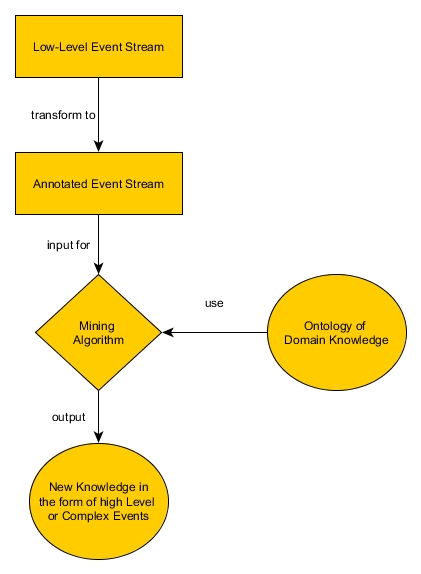
\includegraphics[width=0.25\textwidth]{basicProblemStructure.jpg}
	\caption{Basic Problem Structure}
	\label{fig_basicProblemStructure}
\end{figure}

We follow up with a few definitions about basic terminology and how these will be used in this thesis.

\begin{mydef}
\textbf{Low Level Event} A Low Level Event $v$ is defined as a tuple $l= (t,v_1,...,v_k)$, where $t \in \mathbb{N}^+$ is the timestamp of its occurance and $v_i \in S_i$ is a value reported with the event. $S_i$ is a set of all possible values for the position $i$ which we will not narrow down further here since this obviously depends on the application domain. Common datatypes would of course be real numbers or categorical values.
\end{mydef}

\begin{mydef}
\textbf{Annotated Event} An annotated event $e$ is defined as a tuple $e=(t,T)$, where $t \in \mathbb{N}^+$ is the timestamp and $T \in \Sigma$ is its derived event type. $\Sigma$ is the set of all possible event types, which will sometimes also be referred to as the event type alphabet.
\end{mydef}
Note that this definition assumes that events are instantaneous, which is the usual definition of events (TODO;: is that true?), but there are other variants of event definitions that also allow for events to have a duration (TODO: cite sequences of temporal intervals?). \newline

Given these two definitions we can give a general definition of the first step of the basic setting, the transformation of low level events to annotated events as a function:

\begin{mydef}
\textbf{Transformation Function} A transformation function is a function that takes a low level event $l$ input and maps it to a corresponding annotated event $(t,T)$.
\end{mydef}
Note that this is a very broad definition, since in most cases this function is completely dependent on the domain as well as target event type alphabet and thus by extension the complex events the user is interested in. There are however general methods to automatically transform tuples of real values to annotated events by using bagging (TODO: sources for that). These methods create the target event type alphabet on the fly (depending on the input types). These methods can be useful if we know nothing about the semantics of the low level data or if there is no clear event type alphabet as the target.

\begin{mydef}
\textbf{Annotated Event Stream} An Annotated Event Stream $S$ of length $n$ is defined as a sequence $S=(e_1,...,e_n)$, where all $e_i$ are annotated events and given two events $e_i=(t_i,A)$ and $e_j=(t_j,B)$ we know that $i < j \implies t_i \le t_j$ (the stream is sorted according to the timestamps).
\end{mydef}

The alert reader will have noticed that we assume a total order in the annotated event stream, since we forbid that two consecutive timestamps may have the same value. This means that we do not allow two events to occur concurrently within the stream. For non-distributed streams this basically no restriction, since the events are ordered anyway. If we face a distributed stream (for example in a sensor network) however it might become tricky to fulfill this constraint, since clock synchronization might be an issue. This property is by no means central to the algorithms we will consider, but it does help when analyzing theoretical properties, which is why we assume it for now. \newline
It is also important to note that this definition somewhat simplifies reality, since it assumes that the stream has a certain length, in other words the stream is finite. This is unproblematic if we can assume the following:

\begin{itemize}
	\item $n$ always contains the number of all elements we have seen so far
	\item $n$ gets updated whenever we read a new event
\end{itemize}

However we need to keep this restriction in mind, since the size of the stream will become relevant when determining which episodes are frequent. Most of the time we are not interested in the whole stream, but instead only look at a small window:

\begin{mydef}
\textbf{Time Window} Given an annotated event stream $S$ we define the Time Window $W(S,q,r)$ with $q,r \in \mathbb{N}^+$ and $q < r$ as the subsequence of $S$ that includes all events of $S$ that have a timestamp $t$ where $q \leq t\leq r$. We call $w = r-q+1$ the size of Window $W$.
\end{mydef}

TODO: where to put this:

The form of the ontology is not further specified in this definition since it is very user specific. Common knowledge representations in the area of semantic web technologies are of course RDF-Graphs. The precice process of enriching the data will be discussed later in section TODO.
Fortunately the definition is still sufficient for a general purpose episode mining algorithm, since that algorithm does not require domain knowledge, it just requires the high level event stream. The following definitions are mostly inspiered by \cite{generatingDiverse}.

\subsection{Event Episodes}

Given an annotated stream there are multiple ways to define episodes of events. We will give two different definitions, first a very compact and formal definition and second a longer definition that is a bit more clear and less formal.

\begin{mydef}
\textbf{Episode} An event episode $E$ of length $m$ (also called m-Episode) is defined as a triple: $E = (N_E,{\leq}_{E},g_E)$ where $N_E = \{n_1,...,n_m\}$ is a set of nodes, ${\leq}_{E}$ is a partial order over $N_E$ and $g_E : V_E \rightarrow \Sigma$ is a mapping that maps each node of $N_E$ to an event type. If ${\leq}_{E}$ is a total order we call $E$ a serial episode, if there is no ordering at all we call $E$ a parallel episode. Otherwise we speak of composite episodes.
\end{mydef}

Think of the above definition as a template for concrete occurrences, which we define next:

\begin{mydef}
\textbf{Episode Occurrence} An event episode $E = (N_E,{\leq}_{E},g_E)$ is said to occur in a window $W$ if events of the types that the nodes in $N_E$ are mapped to occur in $W$ in the same order that they occur in the episode. More formally if we are given a sequence of events $S=((t_1,T_1),...,(t_n,T_n))$ (which may be a Time Window, aka. a subsequence of the original Stream) we can define an occurrence of $E$ as an injective Map $h:N_E \rightarrow \{1,...,n\}$, where $g_E(n_i) = T_{h(n_i)}$ and $\forall \, v,w \in V_E : v \;{\leq}_{E}\; w \implies t_{h(v)} \leq t_{h(w)}$ holds.
\end{mydef}

For example given the high level event stream $S = [ (12,A) , (14,B) , (19,C) , (22,A), (34,D) ]$ the Episode $E = (\{n_1,n_2\},\{v_1\; {\leq}_{E} \;n_2\},\{n_1 \rightarrow B,n_2\rightarrow A\}  )$ occurs in window $W(S,14,22)$. \newline \newline

TODO: include the more simple Definition. For now I provide the Link to the paper where the definition is easier to understand (but of course equivalent): http://infolab.stanford.edu/~ullman/mining/episodes.pdf \newline \newline

As already stated many times we are interested in episodes that are frequent. Frequency for episodes however can be defined in different ways and the different definitions have a considerable impact on potential algorithms. The first two definitions, which we will refer to as window based Frequency and Minimal Occurance based Frequency, are mentioned by Zimmermann, when he presents his method for synthetic episode generation \cite{generatingEpisodeDatasets}, but were originally conceived in TODO: include original sources. We refer to the third Definition as the Non-Overlapping Occurrence based Frequency which was suggested by Laxman et al. \cite{fastEpisodeMining}.
\begin{mydef}
\textbf{Episode Frequency - Window based Definition} Given a high level event stream $S$, a fixed window size of $w$ and an Episode $E$, we define the window based frequency $w\_freq(E)$ as the number of windows $W$ with size $w$ of $S$ in which $E$ occurs: $w\_freq(E) = |\,\{W(S,q,r) \mid r-q+1 = w \land E \;occurs\; in\; W \}\,|$.
\end{mydef}

This definition can be confusing at first since it is intended that episode occurrences that are comprised of the exact same events count just as many times as there are windows in which the events appear. If we have a window size of $w=11$ for the above example, we can find the Episode \textit{B after A} in the consecutive windows $W(S,12,22)$, $W(S,13,23)$ and $W(S,14,24)$, which means we will get a frequency of $3$ just for the two events $(14,B)$ and $(22,A)$. This effect obviously increases with the window size. \newline
The second definition does not require a fixed window size to be specified but instead uses the concept of minimal occurrences:

\begin{mydef}
\textbf{Minimal Occurrence} An event episode $E$ is said to occur minimally in a window $W(S,q,r)$ if $E$ occurs in $W$ and there is no subwindow of $W$ in which $E$ also occurs. In this context we also refer to the window $W$ itself as a minimal occurrence of $E$.
\end{mydef}

\begin{mydef}
\textbf{Episode Frequency - Minimal Occurrence based Definition} Given a high level event stream $S$ and an Episode $E$, we define the minimal occurrence based frequency $mo\_freq(E)$ as the number of minimal occurrences of $E$ in $S$.
\end{mydef}

The third definition introduces the concept of non-overlapping occurrences:

\begin{mydef}
\textbf{Non-Overlapping Occurrences} Given a m-Episode $E = (N_E,{\leq}_{E},g_E)$ where $N_E = \{n_1,...,n_m\}$, two occurrences $h_1$ and $h_2$ of $E$ are non-overlapped if either 
\begin{itemize}
	\item $\forall \, n_j \in N_E : h_2(n_1)>h_1(n_j)$ or 
	\item $\forall \, n_j \in N_E : h_1(n_1)>h_2(n_j)$
\end{itemize}
A set of occurrences is non-overlapping if every pair of occurrences in it is non-overlapped.
\end{mydef}

This leads to the Definition:

\begin{mydef}
\textbf{Episode Frequency - Non-Overlapping Occurrences based Definition} Given a high level event stream $S$ and an Episode $E$, we define the non-overlapping occurrence based frequency $noo\_freq(E)$ as cardinality of the largest set of non-overlapped occurrences of $E$ in $S$ \cite{fastEpisodeMining}.
\end{mydef}



When looking at these definitions it is not clear whether any of these is always superior to or more useful than the other since they have different properties. We mention them briefly:

\begin{itemize}
	\item As already mentioned in the above example. The window based frequency counts an episode occurrence that is comprised of the same events in multiple windows. This might especially distort the count if the window size is high and the events in the episode happen with minimal delay between them.
	\item The minimal occurrence based definition of frequency does not suffer from the problem of the previous point
	\item The window based definition has the advantage that it already incorporates a fixed size during which episodes may occur, meaning there can not be episodes that stretch over a time period larger than the fixed window size $w$. This might be beneficial for potential algorithms, since it reduces the search space for episodes. On top of that it is also closer to reality, since episodes normally happen within a small time window (TODO: cite source for this). Of course also the minimal occurrence based definition can be extended to incorporate a maximal time span.
	\item Both definitions do not consider multiple occurrences of an episode in the same time window.
\end{itemize}

TODO: move the above to a separate chapter. Due to the central importance of these definitions we will discuss and compare them in detail in section TODO. \newline \newline


Given these definitions it is the goal of this thesis to develop algorithms that given a stream of high level events will identify frequent episodes in that event stream. Frequent episodes are episodes whose frequency is greater than a user defined threshold, usually relative to the stream length or to the number of inspected windows. Since we are dealing with data-streams the algorithms must have the following properties:

\begin{itemize}
	\item The algorithms must be incremental, since in contrast to classical database scenarios, we might not have all the data at once, but get continuous input instead
	\item The algorithms must require only a single pass over the data, since it might be impossible to store the entire stream, especially since we might be dealing with infinite streams. At best it is possible to store a small window of the most recent data in memory and access that window multiple times.
\end{itemize}


% if have a single appendix:
%\appendix[Proof of the Zonklar Equations]
% or
%\appendix  % for no appendix heading
% do not use \section anymore after \appendix, only \section*
% is possibly needed

% use appendices with more than one appendix
% then use \section to start each appendix
% you must declare a \section before using any
% \subsection or using \label (\appendices by itself
% starts a section numbered zero.)
%


%\appendices
%\section{Proof of the First Zonklar Equation}
%Some text for the appendix.

% use section* for acknowledgement
%\section*{Acknowledgment}


%The authors would like to thank...


% Can use something like this to put references on a page
% by themselves when using endfloat and the captionsoff option.
\ifCLASSOPTIONcaptionsoff
  \newpage
\fi



% trigger a \newpage just before the given reference
% number - used to balance the columns on the last page
% adjust value as needed - may need to be readjusted if
% the document is modified later
%\IEEEtriggeratref{8}
% The "triggered" command can be changed if desired:
%\IEEEtriggercmd{\enlargethispage{-5in}}

% references section

% can use a bibliography generated by BibTeX as a .bbl file
% BibTeX documentation can be easily obtained at:
% http://www.ctan.org/tex-archive/biblio/bibtex/contrib/doc/
% The IEEEtran BibTeX style support page is at:
% http://www.michaelshell.org/tex/ieeetran/bibtex/
%\bibliographystyle{IEEEtran}
% argument is your BibTeX string definitions and bibliography database(s)
%\bibliography{IEEEabrv,../bib/paper}
%
% <OR> manually copy in the resultant .bbl file
% set second argument of \begin to the number of references
% (used to reserve space for the reference number labels box)
\begin{thebibliography}{1}

\bibitem{han2007frequent}
Han, Jiawei, et al. "Frequent pattern mining: current status and future directions." Data Mining and Knowledge Discovery 15.1 (2007): 55-86.

\bibitem{unknownbook}
I could not find the book on google scholar, thus I provide the link to the chapter for now.

\bibitem{predictCritical}
Chen, Jun, and Ratnesh Kumar. "Pattern Mining for Predicting Critical Events from Sequential Event Data Log." WODES. 2014.

\bibitem{anomaly}
Sureka, Ashish. "Kernel Based Sequential Data Anomaly Detection in Business Process Event Logs." arXiv preprint arXiv:1507.01168 (2015).

\bibitem{logcluster}
Vaarandi, Risto, and Mauno Pihelgas. "LogCluster-A Data Clustering and Pattern Mining Algorithm for Event Logs." Network and Service Management (CNSM), 2015 11th International Conference on. IEEE, 2015.

\bibitem{processMining}
Priyadharshini, V., and A. Malathi. "Analysis of Process Mining Model for Software Reliability Dataset using HMM." Indian Journal of Science and Technology 9.4 (2016).

\bibitem{fastFrequentPattern}
Lin, Kawuu W., Sheng-Hao Chung, and Chun-Cheng Lin. "A fast and distributed algorithm for mining frequent patterns in congested networks." Computing (2015): 1-22.

\bibitem{dsms}
Motwani, Rajeev, et al. "Query processing, resource management, and approximation in a data stream management system." CIDR, 2003.

\bibitem{approxfreq}
Manku, Gurmeet Singh, and Rajeev Motwani. "Approximate frequency counts over data streams." Proceedings of the 28th international conference on Very Large Data Bases. VLDB Endowment, 2002.

\bibitem{generatingDiverse}
Zimmermann, Armin. "Generating diverse realistic data sets for episode mining." Data Mining Workshops (ICDMW), 2012 IEEE 12th International Conference on. IEEE, 2012.

\bibitem{closedEpisodeMining}
Zhou, Wenzhi, Hongyan Liu, and Hong Cheng. "Mining closed episodes from event sequences efficiently." Advances in Knowledge Discovery and Data Mining. Springer Berlin Heidelberg, 2010. 310-318.

\bibitem{sequentialPatternMining}
Slimani, Thabet, and Amor Lazzez. "Sequential mining: Patterns and algorithms analysis." arXiv preprint arXiv:1311.0350 (2013).

\bibitem{generatingEpisodeDatasets}
Zimmermann, Armin. "Generating diverse realistic data sets for episode mining." Data Mining Workshops (ICDMW), 2012 IEEE 12th International Conference on. IEEE, 2012.

\bibitem{sequentialPatternMining2}
Zhao, Qiankun, and Sourav S. Bhowmick. "Sequential pattern mining: A survey." ITechnical Report CAIS Nayang Technological University Singapore (2003): 1-26.

\bibitem{fastEpisodeMining}
Laxman, Srivatsan, P. S. Sastry, and K. P. Unnikrishnan. "A fast algorithm for finding frequent episodes in event streams." Proceedings of the 13th ACM SIGKDD international conference on Knowledge discovery and data mining. ACM, 2007.

\end{thebibliography}

% biography section
% 
% If you have an EPS/PDF photo (graphicx package needed) extra braces are
% needed around the contents of the optional argument to biography to prevent
% the LaTeX parser from getting confused when it sees the complicated
% \includegraphics command within an optional argument. (You could create
% your own custom macro containing the \includegraphics command to make things
% simpler here.)
%\begin{biography}[{\includegraphics[width=1in,height=1.25in,clip,keepaspectratio]{mshell}}]{Michael Shell}
% or if you just want to reserve a space for a photo:


% You can push biographies down or up by placing
% a \vfill before or after them. The appropriate
% use of \vfill depends on what kind of text is
% on the last page and whether or not the columns
% are being equalized.

%\vfill

% Can be used to pull up biographies so that the bottom of the last one
% is flush with the other column.
%\enlargethispage{-5in}



% that's all folks
\end{document}


